\documentclass[xcolor=dvipsnames,10pt]{beamer}
% ********** Style prezentation **********

\usepackage{verbatim}
\usepackage{color}
\usepackage{multimedia}
\usepackage{xmpmulti}
\usepackage[absolute,overlay]{textpos} 
\usepackage{listings}
\usepackage{algorithm}
\usepackage{algorithmic}
\usepackage{amsmath}
\usepackage{pifont}
\usepackage{url}
\usepackage{pict2e}
\usepackage{flushend}
\usepackage{graphicx}
\usepackage{pgf}
\usepackage{url}
\usepackage{tikz}
\usetikzlibrary{calc}
\usetikzlibrary{shapes}
\usetikzlibrary{backgrounds}
\usepackage{pgfplots}
\usepackage{pgfplotstable}

\newcommand{\ignore}[1]{}


\lstset{ %
  language=Java,              
  basicstyle=\footnotesize
}

\pgfdeclarelayer{foreground}
\pgfdeclarelayer{background}
\pgfsetlayers{background,main,foreground}

\mode<presentation>
{
	\usetheme{Warsaw}
}
\definecolor{scarlet}{RGB}{200,0,0}
\setbeamercolor{structure}{fg=scarlet}
\addtobeamertemplate{footline}{
\begin{columns}
  \hfill
\includegraphics[height=.75cm]{unl_clear.pdf}\hspace{.5cm}
\end{columns}
\vspace{2mm}
}{\usebeamercolor[bg]{footline}\hfill\raisebox{1mm}[0mm]{\hspace{2mm}}}

\newcommand\x[1]{\ensuremath{\mathit{#1}}}
\newcommand\lrangle[1]{\ensuremath{\langle#1\rangle}}

\def\ON{\ding{52}}
\def\OF{\ding{55}}
\def~{\phantom{0}}

\setbeamertemplate{navigation symbols}{} %remove if navigation symbols are needed
\setbeamersize{text margin left=5mm, text margin right=5mm} % change margin as you wish

\author{Matthew B. Dwyer}

\title[Classic Program Analysis]{Classic Program Analysis}
\subtitle{GTTSE part 2}


\institute{
Department of Computer Science and Engineering\\
University of Nebraska - Lincoln\\
Lincoln, Nebraska USA\\
}

\date{August 2015}

\begin{document}

\begin{frame}
	\titlepage %displays the title page
\end{frame}

\ignore{
\begin{frame}[fragile]
\frametitle{Program Analysis}
\vfill
\vfill
\end{frame}
}

\begin{frame}[fragile]
\frametitle{Program Analysis}
\vfill
For the purpose of this briefing ...
\pause
\vfill
Programs are generators of program traces
\pause
\begin{itemize}
\item a state, $s$, encodes the current program location and the contents of memory, $(l,m)$
\item a statement, $\tau$, is then a transition function on states
\item a trace, $tr$, is dually a sequence of states, $s_0, s_1, \ldots$, or
transitions, $\tau_0, \tau_1, \ldots$
\end{itemize}
\pause
\vfill
For simplicity we will restrict discussion to programs 
\begin{itemize}
\item with a finite set of states 
\item with a finite set of traces
\item with traces of finite length
\end{itemize}
\pause
\vfill
This captures a very large and realistic space of programs
\vfill
\end{frame}

\begin{frame}[fragile]
\frametitle{A (very) simple program}
\vfill
\begin{minipage}{0.5\textwidth}
\begin{lstlisting}
 int y;
\\ 0:
 x = x + 1;
\\ 1:
 if (x < 0) {
\\ 2:
   y = x;
\\ 3:
 } else {
\\ 4:
   y = 0;
\\ 5:
 }
\\ 6:
 x = y + 1;
\\ 7:
\end{lstlisting}
\end{minipage}%
\pause
\begin{minipage}{0.5\textwidth}
``run'' with \texttt{x = -2}\\
\mbox{~}\\
@0: $x = -2, y = 0$\\
\mbox{~}\\
@1: $x = -1, y = 0$\\
\mbox{~}\\
@2: $x = -1, y = 0$\\
\mbox{~}\\
@3: $x = -1, y = -1$\\
\mbox{~}\\
@4: \\
\mbox{~}\\
@5: \\
\mbox{~}\\
@6: $x = -1, y = -1$\\
\mbox{~}\\
@7: $x = 0, y = -1$
\end{minipage}
\vfill
\end{frame}

\begin{frame}[fragile]
\frametitle{A (very) simple program}
\large
\vfill
Even this very simple program has an enormous number of traces
\pause
\[
\mathtt{MAXINT} - \mathtt{MININT} = (2^{31}-1) - (2^{31}) = (2^{32}-1)
\]
\vfill
\pause
When we think about this program we naturally think of two cases
\begin{itemize}
\item values of $x$ that cause the \texttt{if} to take the \textbf{true} branch
\item values of $x$ that cause the \texttt{if} to take the \textbf{false} branch
\end{itemize}
\vfill
\pause
We need two inputs, one for each case, to achieve full path coverage
\vfill
\end{frame}

\begin{frame}[fragile]
\frametitle{Abstraction in Program Analysis}
\large
\vfill
For the simple program we formed an \textit{abstraction} of the values of $x$
\vfill
\pause
This allowed us to collapse $(2^{32}-1)$ traces into $2$
\vfill
\pause
Frameworks for systematically abstracting data in program traces have been studied for nearly 50 years
\begin{itemize}
\item ad-hoc methods in the 1960s were used in the first compilers
\item Kildall's data flow framework was proposed in 1973
\item Boyer, Elspas, Levitt, King, Howden, Clarke developed symbolic execution in 1975-76
\item the Cousot's generalized these ideas in 1977 in the form of \textit{abstract interpretation}
\end{itemize}
\vfill
\end{frame}

\begin{frame}[fragile]
\frametitle{Abstract Interpretation}
\large
\vfill
A non-standard semantics for a program which \textit{abstracts} states
\pause
\vfill
For this talk we'll assume the abstraction is over data values
\begin{itemize}
\item the original values of the program are \textit{concrete}
\item sets of concrete values are replaced by an abstract value
\end{itemize}
\vfill
\pause
We will illustrate the concepts here and provide just a few terms
and definitions
\vfill
\end{frame}

\begin{frame}[fragile]
\frametitle{Abstract Interpretation}
\vfill
\large
Let $\mathcal{C}$ be the set of, concrete, values for the original program
\pause
\vfill
$\mathcal{A}$ defines an \textit{abstract domain} for $\mathcal{C}$ 
if they can be related via a pair of functions
\begin{itemize}
\item $\alpha : \mathcal{C} \mapsto \mathcal{A}$, the abstraction function
\item $\gamma : \mathcal{A} \mapsto 2^\mathcal{C}$, the concretization functoin
\end{itemize}
\vfill
such that
\[
\forall c \in \mathcal{C} : \alpha(c) \in \mathcal{A} \wedge c \in \gamma(\alpha(c))
\]
\vfill
\end{frame}


\begin{frame}[fragile]
\frametitle{Abstract domains}
\large
\vfill
Abstract domains are usually partially ordered, $\sqsupseteq$, so that
\pause
\vfill
\[
\forall a,a' \in \mathcal{A} :  a \sqsupseteq a' \implies \gamma(a) \supseteq \gamma(a')
\]
\vfill
\pause
Moreover they usually define a meet-semilattice
\begin{itemize}
\item they have a binary meet (greatest lower bound) operator, $\sqcap$
\item they have a maximal, $\top \in \mathcal{A}$ 
\end{itemize}
such that 
\vfill
\[
\forall a \in \mathcal{A} : a \sqcap \top = a
\]
\vfill
\end{frame}


\begin{frame}[fragile]
\frametitle{An extreme abstract domain}
\large
\vfill
\ignore{
No abstraction is an abstraction
\pause
\vfill
\begin{gather*}
\mathcal{A_{\mathit{identity}}} = \mathcal{C} \cup \{\ \top \}\\
\alpha_{identity} = \lambda x.x\\
\gamma_{identity} = \lambda x.(x=\top ? 2^{\mathcal{C}} : x)\\
\forall x \not= y : x \sqcap y = \top, \forall x : x \sqcap x = x
\end{gather*}
}
\vfill
The \textit{forgetful} abstraction 
\vfill
\begin{gather*}
\mathcal{A_{\mathit{forget}}} = \{ \top \}\\
\alpha_{forget} = \lambda x . \top\\
\gamma_{forget} = \lambda x . \mathcal{C}\\
\top \sqcap \top = \top
\end{gather*}
\vfill
\end{frame}

\begin{frame}[fragile]
\frametitle{The \textit{interval} abstract domain}
\large
\vfill
Represent a set of consecutive values in the concrete domain by their endpoints
\begin{itemize}
\item in terms of interval arithmetic these are \textit{closed intervals}
\end{itemize}
\vfill
\pause
\begin{gather*}
\mathcal{C} = \mathtt{int}\\
\mathcal{A_{\mathit{interval}}} = \{ [x,y] \mid x,y \in \mathcal{C} \wedge x \le y \} \cup \{ [-\infty, \infty] \}\\
\mathrm{, where } \; \forall x : -\infty < x \wedge x < \infty\\
\alpha_{interval} = \lambda x.[x,x]\\
\gamma_{interval} = \lambda [x,y].\{ z \mid x \le z \wedge z \le y\}\\
[x,y] \sqcap [x',y'] = [min(x,x'),max(y,y')]
\end{gather*}
\vfill
\end{frame}


\begin{frame}[fragile]
\frametitle{The \textit{interval} abstract domain}
\large
\vfill
\begin{tikzpicture}
  \node (top) at (0,7) {$[-\infty,\infty]$};
  \node (top1) at (-1,6) {};
  \node (top2) at (0,6) {};
  \node (top3) at (1,6) {};

  \draw[dashed] (top) -- (top1);
  \draw[dashed] (top) -- (top2);
  \draw[dashed] (top) -- (top3);

  \node (minf3) at (-2,5) {};
  \node (minf2) at (-3,4) {$[-\infty,1]$};
  \node (minf1) at (-4,3) {$[-\infty,0]$};
  \node (minf0) at (-5,2) {$[-\infty,-1]$};
  \node (minfm1) at (-6,1) {};

  \draw[dashed] (minf3) -- (minf2);
  \draw (minf2) -- (minf1);
  \draw (minf1) -- (minf0);
  \draw[dashed] (minf0) -- (minfm1);

  \node (thrinf) at (2,5) {};
  \node (twoinf) at (3,4) {$[-1,\infty]$};
  \node (oneinf) at (4,3) {$[0,\infty]$};
  \node (zeroinf) at (5,2) {$[1,\infty]$};
  \node (m1inf) at (6,1) {};

  \draw[dashed] (thrinf) -- (twoinf);
  \draw (twoinf) -- (oneinf);
  \draw (oneinf) -- (zeroinf);
  \draw[dashed] (m1inf) -- (zeroinf);

  \node (m22) at (0,4) {$[-2,2]$};

  \node (m21) at (-1,3) {$[-2,1]$};
  \node (m12) at (1,3) {$[-1,2]$};

  \node (m20) at (-2,2) {$[-2,0]$};
  \node (m11) at (0,2) {$[-1,1]$};
  \node (zero2) at (2,2) {$[0,2]$};

  \node (m2m1) at (-3,1) {$[-2,-1]$};
  \node (m10) at (-1,1) {$[-1,0]$};
  \node (zero1) at (1,1) {$[0,1]$};
  \node (one2) at (3,1) {$[1,2]$};

  \node (m2m2) at (-4,0) {$[-2,-2]$};
  \node (m1m1) at (-2,0) {$[-1,-1]$};
  \node (zero0) at (0,0) {$[0,0]$};
  \node (one1) at (2,0) {$[1,1]$};
  \node (two2) at (4,0) {$[2,2]$};

  \draw (m2m2) -- (m2m1);
  \draw (m1m1) -- (m2m1);
  \draw (m1m1) -- (m10);
  \draw (zero0) -- (m10);
  \draw (zero0) -- (zero1);
  \draw (one1) -- (zero1);
  \draw (one1) -- (one2);
  \draw (two2) -- (one2);

  \draw (m2m1) -- (m20);
  \draw (m10) -- (m20);
  \draw (m10) -- (m11);
  \draw (zero1) -- (m11);
  \draw (zero1) -- (zero2);
  \draw (one2) -- (zero2);

  \draw (m20) -- (m21);
  \draw (m11) -- (m21);
  \draw (m11) -- (m12);
  \draw (zero2) -- (m12);

  \draw (m21) -- (m22);
  \draw (m12) -- (m22);

\end{tikzpicture}
\vfill
\end{frame}



\begin{frame}[fragile]
\frametitle{A \textit{predicate} abstraction}
\large
\vfill
Define a set of predicates, $\mathcal{P}$,  that are characteristic functions for subsets of $\mathcal{C}$
\begin{itemize}
\item in many frameworks the set of predicates covers $\mathcal{C}$
\item predicates need not be disjoint, i.e., $\gamma(p) \cap \gamma(q) \not= \emptyset$
\end{itemize}
\vfill
\pause
\begin{gather*}
\mathcal{A_{\mathit{pred}}} = \{ \phi \mid \forall F \subseteq \mathcal{P} : \phi = \bigvee_{p \in F} \} \cup \{ \top \} \mathrm{, where} \; \top=\mathit{true}\\
\alpha_{pred} = \lambda x.\bigvee_{p' \in \{ p \mid p \in \mathcal{P} \wedge p(x)\}}\\
\gamma_{pred} = \lambda \phi.\{ x \mid \phi(x) \}\\
\end{gather*}
\vfill
\pause
For example, the \textit{signs} abstraction
\begin{itemize}
\item $\mathcal{P} = \{ \lambda x.x<0, \lambda x.x=0, \lambda x.x>0 \}$
\item $\le 0$ is encoded by the disjunction $\lambda x.x<0 \wedge \lambda x.x=0$
\end{itemize}
\vfill
\end{frame}

\begin{frame}[fragile]
\frametitle{An abstract domain is not enough}
\large
\vfill
We must define the meaning of program statements over that domain
\pause
\vfill
For a statement $\tau$, its semantics over $\mathcal{A}$ is given by $\tau^\#$
\[
\forall c, c' \in \mathcal{C} : \tau(c) = c' \implies \tau^\#(\alpha(c)) \sqsupseteq \alpha(c')
\]
\pause
\vfill
This implies the classic overapproximating correctness
relation for abstracted program statements:
\[
\tau^\# \sqsupseteq \alpha \circ \tau \circ \gamma
\]
\vfill
\end{frame}

\begin{frame}[fragile]
\frametitle{An abstract domain is not enough}
\large
\vfill
Historically developing abstract transformers was creative and costly 
\pause
\vfill
For each operation \textit{lift} it to $\mathcal{A}$, e.g.,
$[x,y] + [x',y'] = [x+x',y+y']$
\pause
\vfill
Branching statements are interesting
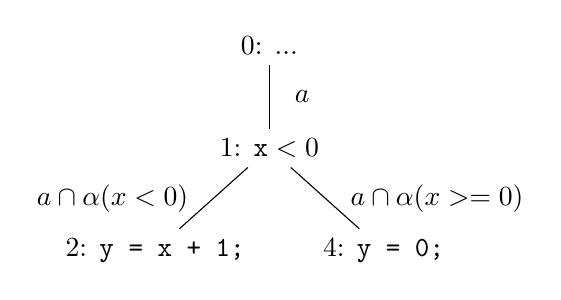
\begin{tikzpicture}[scale=0.6]
  \node {0: ...}
     child {
       node[xshift=0mm, yshift=-4mm] {1: $\mathtt{x} < 0$}
       child {
         node[xshift=-10mm, yshift=-4mm] {2: \texttt{y = x + 1;}}
         edge from parent node[left, xshift=-2mm] {$a \cap \alpha(x < 0)$}
       }
       child {
         node[xshift=10mm, yshift=-4mm] {4: \texttt{y = 0;}}
         edge from parent node[right, xshift=2mm] {$a \cap \alpha(x >= 0)$}
       }
       edge from parent node[right, xshift=2mm] {$a$}
     };
\end{tikzpicture}
\pause
\vfill
Loops require fixpoint computations (and help with convergence, i.e., widening)
\vfill
\end{frame}

\begin{frame}[fragile]
\frametitle{An abstract domain is not enough}
\large
\vfill
Thakur, Elder and Reps in their SAS 2012 paper ``Bilateral algorithm for symbolic abstraction''  
\begin{itemize}
\item from an abstract domain given as a set of predicates
\item compute the \textit{best} abstract transformer, i.e., 
$\tau^\# = \alpha \circ \tau \circ \gamma$
\item they use an SMT solver to iteratively approximate the transformer
\item soundly tolerates SMT solver failures
\end{itemize}
\vfill
\end{frame}


\begin{frame}[fragile]
\frametitle{Abstract values and statements define abstract traces}
\vfill
\begin{minipage}{0.3\textwidth}
\large
\begin{lstlisting}
 int y;
\\ 0:
 x = x + 1;
\\ 1:
 if (x < 0) {
\\ 2:
   y = x;
\\ 3:
 } else {
\\ 4:
   y = 0;
\\ 5:
 }
\\ 6:
 x = y + 1;
\\ 7:
\end{lstlisting}
\end{minipage}%
\pause
\begin{minipage}{0.6\textwidth}
``abstractly interpret'' with $\mathcal{A_{\mathrm{interval}}}$ and $-10 \le x \le 10$\\
\mbox{~}\\
@0: $x = [-10,10], y = [0,0]$\\
\mbox{~}\\
@1: $x = [-9,11], y = [0,0]$\\
\mbox{~}\\
@2: $x = [-9,-1], y = [0,0]$\\
\mbox{~}\\
@3: $x = [-9,-1], y = [-9,-1]$\\
\mbox{~}\\
@4: \\
\mbox{~}\\
@5: \\
\mbox{~}\\
@6: $x = [-9,-1], y = [-9,-1]$\\
\mbox{~}\\
@7: $x = [-8,0], y = [-9,-1]$
\vfill
\end{minipage}
\end{frame}

\begin{frame}[fragile]
\frametitle{Some observations ...}
\large
\vfill
\pause
We started not from a single value for \texttt{x}, but from a set of values
\vfill
\pause
That set was encoded using the abstract domain
\vfill
\pause
The statements of the program were \textit{lifted} to operate on the abstract domain
\vfill
\pause
If the semantics of a statement can yield different results for elements of a set, i.e., $\gamma(s)$, then all results must be reflected
\pause
\vfill
In our example, this happens
\begin{itemize}
\item $x = [-9,11]$ on entry to \texttt{if (x<0)}
\item the true branch \textbf{and} the false branch can be taken
\item the effect of all paths leading to a location is reflected through $\sqcap$
\end{itemize}
\vfill
\end{frame}

\begin{frame}[fragile]
\frametitle{Abstract values and statements define abstract traces}
\vfill
\begin{minipage}{0.25\textwidth}
\begin{lstlisting}
 int y;
\\ 0:
 x = x + 1;
\\ 1:
 if (x < 0) {
\\ 2:
   y = x;
\\ 3:
 } else {
\\ 4:
   y = 0;
\\ 5:
 }
\\ 6:
 x = y + 1;
\\ 7:
\end{lstlisting}
\end{minipage}%
\hfill
\begin{minipage}{0.3\textwidth}
\small
true branch with $\mathcal{A_{\mathrm{interval}}}$\\
\mbox{~}\\
@0: $x = [-10,10],$\\ 
\mbox{~~~~}$y = [0,0]$\\
@1: $x = [-9,11],$\\
\mbox{~~~~}$y = [0,0]$\\
@2: $x = [-9,-1],$\\
\mbox{~~~~}$y = [0,0]$\\
@3: $x = [-9,-1],$\\
\mbox{~~~~}$y = [-9,-1]$\\
@4: \\
\mbox{~}\\
@5: \\
\mbox{~}\\
@6: $x = [-9,-1],$\\
\mbox{~~~~}$y = [-9,-1]$\\
@7: $x = [-8,0],$\\
\mbox{~~~~}$y = [-9,-1]$
\end{minipage}%
\hfill
\begin{minipage}{0.3\textwidth}
\small
false branch with $\mathcal{A_{\mathrm{interval}}}$\\
\mbox{~}\\
@0: $x = [-10,10],$\\
\mbox{~~~~}$y = [0,0]$\\
@1: $x = [-9,11],$\\
\mbox{~~~~}$y = [0,0]$\\
@2: \\
\mbox{~}\\
@3: \\
\mbox{~}\\
@4: $x = [0,11],$\\
\mbox{~~~~}$y = [0,0]$\\
@5: $x = [0,11],$\\
\mbox{~~~~}$y = [0,0]$\\
@6: $x = [0,11],$\\
\mbox{~~~~}$y = [0,0]$\\
@7: $x = [1,1],$\\
\mbox{~~~~}$y = [0,0]$
\end{minipage}
\vfill
\end{frame}

\begin{frame}[fragile]
\frametitle{Abstracting traces with $\mathcal{A}_{\mathrm{interval}}$}
\vfill
\begin{minipage}{0.25\textwidth}
\begin{lstlisting}
 int y;
\\ 0:
 x = x + 1;
\\ 1:
 if (x < 0) {
\\ 2:
   y = x;
\\ 3:
 } else {
\\ 4:
   y = 0;
\\ 5:
 }
\\ 6:
 x = y + 1;
\\ 7:
\end{lstlisting}
\end{minipage}%
\hfill
\begin{minipage}{0.6\textwidth}
\small
\mbox{~}\\
@0: $x = [-10,10],$ \mbox{~~~~~~~~~~} ...\\ 
\mbox{~~~~}$y = [0,0]$ \mbox{~~~~~~~~~~~~~~} ...\\
@1: $x = [-9,11],$ \mbox{~~~~~~~~~~~} ...\\
\mbox{~~~~}$y = [0,0]$ \mbox{~~~~~~~~~~~~~~} ...\\
@2: $x = [-9,-1],$ \mbox{~~~~~~~~~~} ...\\
\mbox{~~~~}$y = [0,0]$ \mbox{~~~~~~~~~~~~~~} ...\\
@3: $x = [-9,-1],$ \mbox{~~~~~~~~~~} ...\\
\mbox{~~~~}$y = [-9,-1]$ \mbox{~~~~~~~~~~} ...\\
@4:\mbox{~~~~~~~~~~~~~~~~~~~~} $x = [0,11],$\\
   \mbox{~~~~~~~~~~~~~~~~~~~~~~~} $y = [0,0]$\\
@5:\mbox{~~~~~~~~~~~~~~~~~~~~} $x = [0,11],$\\
   \mbox{~~~~~~~~~~~~~~~~~~~~~~~} $y = [0,0]$\\
@6: \onslide<2-3>{\textcolor{red}{$x = [-9,-1] \sqcap [0,11] = [-9,11]$}}\\
\mbox{~~~~}\onslide<2-3>{\textcolor{red}{$y = [-9,-1] \sqcap [0,0] = [-9,0]$}}\\
@7: \onslide<3>{\textcolor{red}{$x = [-8,1],$}}\\
\mbox{~~~~}\onslide<3>{\textcolor{red}{$y = [-9,0]$}}
\end{minipage}%
\vfill
\end{frame}

\ignore{
\begin{frame}[fragile]
\frametitle{Abstracting traces with $\mathcal{A}_{\mathrm{pred}}$}
\vfill
\begin{minipage}{0.25\textwidth}
\begin{lstlisting}
 int y;
\\ 0:
 x = x + 1;
\\ 1:
 if (x < 0) {
\\ 2:
   y = x;
\\ 3:
 } else {
\\ 4:
   y = 0;
\\ 5:
 }
\\ 6:
 x = y + 1;
\\ 7:
\end{lstlisting}
\end{minipage}%
\hfill
\pause
\begin{minipage}{0.6\textwidth}
\footnotesize
true branch with $\mathcal{A_{\mathrm{pred}}}$\\
\mbox{~}\\
@0: $p_{lz}(x) \vee p_{ez}(x) \vee p_{gz}(x), p_{ez}(y)$\\
\mbox{~}\\
@1: $p_{lz}(x) \vee p_{ez}(x) \vee p_{gz}(x), p_{ez}(y)$\\
\mbox{~}\\
@2: $p_{lz}(x), p_{ez}(y)$\\
\mbox{~}\\
@3: $p_{lz}(x), p_{lz}(y)$\\
\mbox{~}\\
@4: \mbox{~~~~~~~~~~~~~~~~~~~~~~~~~}$p_{ez}(x) \vee p_{gz}(x), p_{ez}(y)$\\
\mbox{~}\\
@5: \mbox{~~~~~~~~~~~~~~~~~~~~~~~~~}$p_{ez}(x) \vee p_{gz}(x), p_{ez}(y)$\\
\mbox{~}\\
@6: $p_{lz}(x), p_{lz}(y) \sqcap p_{ez}(x) \vee p_{gz}(x), p_{ez}(y) =$\\
\mbox{~~~} $p_{lz}(x) \vee p_{ez}(x) \vee p_{gz}(x), p_{lz}(y) \vee p_{ez}(y)$\\
@7: $p_{lz}(x) \vee p_{ez}(x) \vee p_{gz}(x),$\\
\mbox{~~~} $p_{lz}(y) \vee p_{ez}(y) \vee p_{gz}(y)$
\end{minipage}%
\vfill
\end{frame}
}

\begin{frame}[fragile]
\frametitle{Some observations ...}
\vfill
Differing domains can give rise to different analysis results
\vfill
A good choice of domain is subtle and will take into account 
the semantics of the program
\vfill
To address this the past decade has seen many methods that 
\begin{itemize}
\item develop sophisticated parameterized domains (e.g., PARMA's parameterized polyhedra)
\item iteratively refine the abstract domain (e.g., CEGAR-based predicate abstraction)
\end{itemize}
\vfill
As we will see these are directions that recent work on probabilistic analysis has begun to adopt
\vfill
\end{frame}

\ignore{
\begin{frame}[fragile]
\frametitle{Model checking}
\vfill
I could give an entire briefing on this.
\pause
\vfill
The key points are ...
\begin{itemize}
\item program behavior is represented in a state transition system
\item all behaviors are computed by means of a fixpoint computation
\item e.g., through DFS on the state space the transition system
\item e.g., through powering the transition relation
\end{itemize}
\vfill
\end{frame}
}

\begin{frame}[fragile]
\frametitle{Data flow analysis}
\large
\vfill
Fantastic paper published in POPL in 1999 by David Schmidt
\vfill
He describes how data flow analysis ...
\begin{itemize}
\item which has been used since the 1960s in optimizing compilers
\item which is often viewed as a bit \textit{shakier} in its foundations
\end{itemize}
can be viewed as model checking of abstract interpretations
\vfill
abstract interpretation is used to abstract traces and defines $\sqcap$
\vfill
model checking computes fixed points to merge traces using $\sqcap$
\vfill
\end{frame}

\begin{frame}[fragile]
\frametitle{Data flow analysis}
\vfill
\begin{minipage}{0.45\textwidth}
\begin{algorithm}[H]
\caption{{\tt dfa}$(\iota,a)$}
\label{alg-dfa}
\begin{algorithmic}
 \STATE $a[l_0] \gets \iota$
 \STATE $\forall l \not= l_0 : a[l] \gets \top$
 \STATE $w \gets \{l_0\}$
 \WHILE{$w \not= \emptyset$}
   \STATE $l \gets remove(w)$
   \STATE $t \gets {op(l)}^{\#}(a[l])$
   \FOR{$l' \in succ(l)$}
     \STATE $a[l'] \gets (o \gets a[l']) \sqcap t$
     \IF{$a[l'] \not= o$}
       \STATE $w \gets w \cup \{l'\}$
     \ENDIF
   \ENDFOR
 \ENDWHILE
\end{algorithmic}
\end{algorithm}
\end{minipage}%
\hfill
\begin{minipage}{0.53\textwidth}
\vfill
$a$ is a map that stores, for each location $l$, the abstracted memory state
\begin{itemize}
\item $\iota$ is the abstraction of the initial state
\end{itemize}
\vfill
\mbox{~}\\
Whenever a node receives ``new'' information it applies $\sqcap$
\begin{itemize}
\item new information means that $\gamma(a_{new}[l]) - \gamma(a[l]) \not= \emptyset$
\end{itemize}
\vfill
\mbox{~}\\
Iterate until no new information is produced
\vfill
\end{minipage}
\vfill
\end{frame}

\begin{frame}[fragile]
\frametitle{Assessment : Data Flow Analysis}
\vfill
Designed to overapproximate program behavior, i.e., reachable states
\vfill
These analyses are intended to be \textit{sound} - if the analysis says it is true then it is true of the program's behavior
\vfill
Many ways to boost precision
\begin{itemize}
\item \textit{sensitivity}: flow, path, calling-context, synchronization, ...
\item products of abstract domains: direct, smash, reduced, ...
\end{itemize}
\vfill
Tool support
\begin{itemize}
\item SOOT (McGill), Wala (IBM), PRISM (GaTech), many more 
\end{itemize}
\vfill
Used in practice all over the place
\begin{itemize}
\item pretty much every compiler and IDE, many commercial tools
\end{itemize}
\vfill
\end{frame}

\begin{frame}[fragile]
\frametitle{Symbolic execution}
\vfill
Uses a symbolic abstraction like predicate abstraction
\begin{itemize}
\item a logical formula describes the program state
\item stores a map from program locations to symbolic expressions over program input variables
\item records a \textit{path condition} giving constraints on branch outcomes in terms of input variables
\end{itemize}
\vfill
There is no guarantee to characterize abstract states reached by \textbf{all} traces
\begin{itemize}
\item analysis is path-sensitive 
\item path-explosion limits ability to cover program behavior
\item some paths will be skipped: heuristically, based on resource constraints
\end{itemize}
\vfill
\end{frame}

\begin{frame}{Basic symbolic execution algorithm} 
\vfill
\begin{minipage}{0.5\textwidth}
\begin{algorithm}[H]
\caption{{\tt symx}$(l,m,pc)$}
\label{alg-symexe}
\begin{algorithmic}
\IF{$\x{stoppingPath}(pc)$}
 \RETURN
 \ENDIF
 \WHILE{$\neg \x{branch}(l)$}
   \STATE $m \gets \x{op}(l)(m)$
   \STATE $l \gets \x{succ}(l)$
 \ENDWHILE

 \STATE $c \gets \x{cond}(l)(m)$

 \IF{SAT$(pc \wedge c)$}
   \STATE {\tt symx}$(\x{succ_t}(l), m, pc \wedge c)$
 \ENDIF

 \IF{SAT$(pc \wedge \neg c)$}
   \STATE {\tt symx}$(\x{succ_f}(l), m, pc \wedge \neg c)$
 \ENDIF
\end{algorithmic}
\end{algorithm}
\end{minipage}%
\begin{minipage}{0.5\textwidth}
\vfill
\mbox{~}\\
During sequences of statements accumulate the symbolic map $m$
\vfill
\mbox{~}\\
When a branch is encountered check branch outcomes for feasibility
\begin{itemize}
\item If the logical encoding of a path is satisfiable, then it is feasible
\end{itemize}
\vfill
\mbox{~}\\
Recursively explore the feasible branch outcomes
\vfill
\end{minipage}%
\vfill
\end{frame}

\begin{frame}[fragile]
\frametitle{Symbolic execution of simple example}
\vfill
\begin{minipage}{0.3\textwidth}
\begin{lstlisting}
 int y;
\\ 0:
 x = x + 1;
\\ 1:
 if (x < 0) {
\\ 2:
   y = x;
\\ 3:
 } else {
\\ 4:
   y = 0;
\\ 5:
 }
\\ 6:
 x = y + 1;
\\ 7:
\end{lstlisting}
\end{minipage}%
\begin{minipage}{0.5\textwidth}
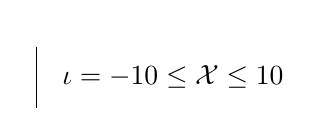
\begin{tikzpicture}[scale=0.6]
  \node {}
    child {
     %node {0: $\mathtt{x}=\mathcal{X}+1$}
     %child {
     %  node[xshift=0mm, yshift=-4mm] {1: $\mathtt{x} < 0$}
     %  child {
     %    node[xshift=-10mm, yshift=-4mm] {2: $\mathtt{y} = \mathcal{X}+1$}
     %    child {
     %      node[xshift=0mm, yshift=-4mm] {6: $\mathtt{x} = \mathcal{X}+1+1$}
     %      edge from parent node[left, xshift=-2mm] {$\mathcal{X} + 1 < 0$}
     %    }
     %    edge from parent node[left, xshift=-2mm] {$\mathcal{X} + 1 < 0$}
     %  }
     %  child {
     %    node[xshift=10mm, yshift=-4mm] {4: $\mathtt{y} = 0$}
     %    child {
     %      node[xshift=0mm, yshift=-4mm] {6: $\mathtt{x} = 0$}
     %      edge from parent node[right, xshift=2mm] {$\neg (\mathcal{X} + 1 < 0)$}
     %    }
     %    edge from parent node[right, xshift=2mm] {$\neg (\mathcal{X} + 1 < 0)$}
     %  }
     %  edge from parent node[right, xshift=2mm] {$\iota$}
     %}
     edge from parent node[right, xshift=2mm] {$\iota = -10 \le \mathcal{X} \le 10$}
    };
\end{tikzpicture}
\end{minipage}
\vfill
\end{frame}


\begin{frame}[fragile]
\frametitle{Symbolic execution of simple example}
\vfill
\begin{minipage}{0.3\textwidth}
\begin{lstlisting}
 int y;
\\ 0:
 x = x + 1;
\\ 1:
 if (x < 0) {
\\ 2:
   y = x;
\\ 3:
 } else {
\\ 4:
   y = 0;
\\ 5:
 }
\\ 6:
 x = y + 1;
\\ 7:
\end{lstlisting}
\end{minipage}%
\begin{minipage}{0.5\textwidth}
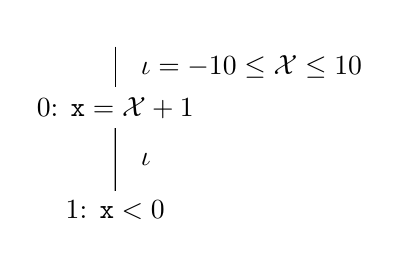
\begin{tikzpicture}[scale=0.6]
  \node {}
    child {
     node {0: $\mathtt{x}=\mathcal{X}+1$}
     child {
       node[xshift=0mm, yshift=-4mm] {1: $\mathtt{x} < 0$}
       %child {
       %  node[xshift=-10mm, yshift=-4mm] {2: $\mathtt{y} = \mathcal{X}+1$}
       %  child {
       %    node[xshift=0mm, yshift=-4mm] {6: $\mathtt{x} = \mathcal{X}+1+1$}
       %    edge from parent node[left, xshift=-2mm] {$\mathcal{X} + 1 < 0$}
       %  }
       %  edge from parent node[left, xshift=-2mm] {$\mathcal{X} + 1 < 0$}
       %}
       %child {
       %  node[xshift=10mm, yshift=-4mm] {4: $\mathtt{y} = 0$}
       %  child {
       %    node[xshift=0mm, yshift=-4mm] {6: $\mathtt{x} = 0$}
       %    edge from parent node[right, xshift=2mm] {$\neg (\mathcal{X} + 1 < 0)$}
       %  }
       %  edge from parent node[right, xshift=2mm] {$\neg (\mathcal{X} + 1 < 0)$}
       %}
       edge from parent node[right, xshift=2mm] {$\iota$}
     }
     edge from parent node[right, xshift=2mm] {$\iota = -10 \le \mathcal{X} \le 10$}
    };
\end{tikzpicture}
\end{minipage}
\vfill
\end{frame}

\begin{frame}[fragile]
\frametitle{Symbolic execution of simple example}
\vfill
\begin{minipage}{0.3\textwidth}
\begin{lstlisting}
 int y;
\\ 0:
 x = x + 1;
\\ 1:
 if (x < 0) {
\\ 2:
   y = x;
\\ 3:
 } else {
\\ 4:
   y = 0;
\\ 5:
 }
\\ 6:
 x = y + 1;
\\ 7:
\end{lstlisting}
\end{minipage}%
\begin{minipage}{0.5\textwidth}
\begin{tikzpicture}[scale=0.6]
  \node {}
    child {
     node {0: $\mathtt{x}=\mathcal{X}+1$}
     child {
       node[xshift=0mm, yshift=-4mm] {1: $\mathtt{x} < 0$}
       child {
         node[xshift=-10mm, yshift=-4mm] {2: $\mathtt{y} = \mathcal{X}+1$}
         %child {
         %  node[xshift=0mm, yshift=-4mm] {6: $\mathtt{x} = \mathcal{X}+1+1$}
         %  edge from parent node[left, xshift=-2mm] {$\mathcal{X} + 1 < 0$}
         %}
         edge from parent node[left, xshift=-2mm] {$\iota \wedge \mathcal{X} + 1 < 0$}
       }
       %child {
       %  node[xshift=10mm, yshift=-4mm] {4: $\mathtt{y} = 0$}
       %  child {
       %    node[xshift=0mm, yshift=-4mm] {6: $\mathtt{x} = 0$}
       %    edge from parent node[right, xshift=2mm] {$\neg (\mathcal{X} + 1 < 0)$}
       %  }
       %  edge from parent node[right, xshift=2mm] {$\neg (\mathcal{X} + 1 < 0)$}
       %}
       edge from parent node[right, xshift=2mm] {$\iota$}
     }
     edge from parent node[right, xshift=2mm] {$\iota = -10 \le \mathcal{X} \le 10$}
    };
\end{tikzpicture}
\end{minipage}
\vfill
\end{frame}

\begin{frame}[fragile]
\frametitle{Symbolic execution of simple example}
\vfill
\begin{minipage}{0.3\textwidth}
\begin{lstlisting}
 int y;
\\ 0:
 x = x + 1;
\\ 1:
 if (x < 0) {
\\ 2:
   y = x;
\\ 3:
 } else {
\\ 4:
   y = 0;
\\ 5:
 }
\\ 6:
 x = y + 1;
\\ 7:
\end{lstlisting}
\end{minipage}%
\begin{minipage}{0.5\textwidth}
\begin{tikzpicture}[scale=0.6]
  \node {}
    child {
     node {0: $\mathtt{x}=\mathcal{X}+1$}
     child {
       node[xshift=0mm, yshift=-4mm] {1: $\mathtt{x} < 0$}
       child {
         node[xshift=-10mm, yshift=-4mm] {2: $\mathtt{y} = \mathcal{X}+1$}
         child {
           node[xshift=0mm, yshift=-4mm] {6: $\mathtt{x} = \mathcal{X}+1+1$}
           edge from parent node[left, xshift=-2mm] {$\iota \wedge \mathcal{X} + 1 < 0$}
         }
         edge from parent node[left, xshift=-2mm] {$\iota \wedge \mathcal{X} + 1 < 0$}
       }
       %child {
       %  node[xshift=10mm, yshift=-4mm] {4: $\mathtt{y} = 0$}
       %  child {
       %    node[xshift=0mm, yshift=-4mm] {6: $\mathtt{x} = 0$}
       %    edge from parent node[right, xshift=2mm] {$\neg (\mathcal{X} + 1 < 0)$}
       %  }
       %  edge from parent node[right, xshift=2mm] {$\neg (\mathcal{X} + 1 < 0)$}
       %}
       edge from parent node[right, xshift=2mm] {$\iota$}
     }
     edge from parent node[right, xshift=2mm] {$\iota = -10 \le \mathcal{X} \le 10$}
    };
\end{tikzpicture}
\end{minipage}
\vfill
\end{frame}

\begin{frame}[fragile]
\frametitle{Symbolic execution of simple example}
\vfill
\begin{minipage}{0.3\textwidth}
\begin{lstlisting}
 int y;
\\ 0:
 x = x + 1;
\\ 1:
 if (x < 0) {
\\ 2:
   y = x;
\\ 3:
 } else {
\\ 4:
   y = 0;
\\ 5:
 }
\\ 6:
 x = y + 1;
\\ 7:
\end{lstlisting}
\end{minipage}%
\begin{minipage}{0.5\textwidth}
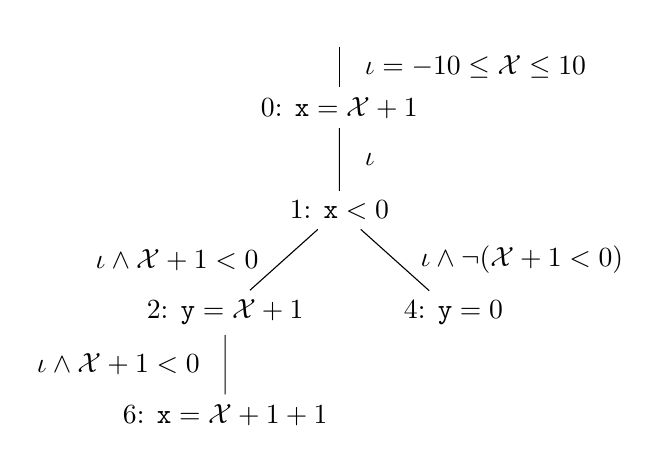
\begin{tikzpicture}[scale=0.6]
  \node {}
    child {
     node {0: $\mathtt{x}=\mathcal{X}+1$}
     child {
       node[xshift=0mm, yshift=-4mm] {1: $\mathtt{x} < 0$}
       child {
         node[xshift=-10mm, yshift=-4mm] {2: $\mathtt{y} = \mathcal{X}+1$}
         child {
           node[xshift=0mm, yshift=-4mm] {6: $\mathtt{x} = \mathcal{X}+1+1$}
           edge from parent node[left, xshift=-2mm] {$\iota \wedge \mathcal{X} + 1 < 0$}
         }
         edge from parent node[left, xshift=-2mm] {$\iota \wedge \mathcal{X} + 1 < 0$}
       }
       child {
         node[xshift=10mm, yshift=-4mm] {4: $\mathtt{y} = 0$}
         %child {
         %  node[xshift=0mm, yshift=-4mm] {6: $\mathtt{x} = 0$}
         %  edge from parent node[right, xshift=2mm] {$\neg (\mathcal{X} + 1 < 0)$}
         %}
         edge from parent node[right, xshift=2mm] {$\iota \wedge \neg (\mathcal{X} + 1 < 0)$}
       }
       edge from parent node[right, xshift=2mm] {$\iota$}
     }
     edge from parent node[right, xshift=2mm] {$\iota = -10 \le \mathcal{X} \le 10$}
    };
\end{tikzpicture}
\end{minipage}
\vfill
\end{frame}

\begin{frame}[fragile]
\frametitle{Symbolic execution of simple example}
\vfill
\begin{minipage}{0.3\textwidth}
\begin{lstlisting}
 int y;
\\ 0:
 x = x + 1;
\\ 1:
 if (x < 0) {
\\ 2:
   y = x;
\\ 3:
 } else {
\\ 4:
   y = 0;
\\ 5:
 }
\\ 6:
 x = y + 1;
\\ 7:
\end{lstlisting}
\end{minipage}%
\begin{minipage}{0.5\textwidth}
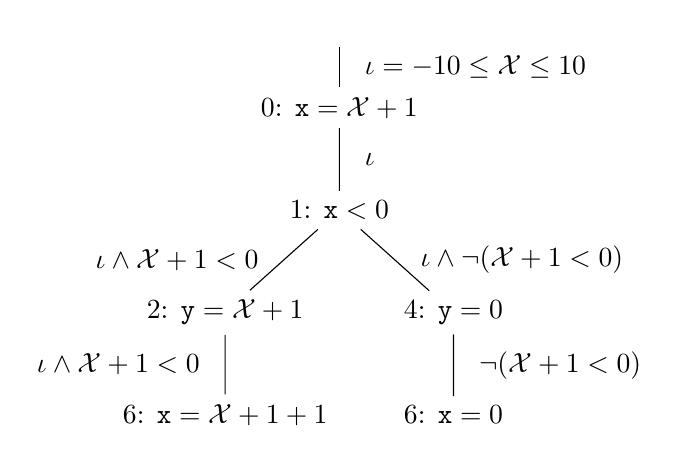
\begin{tikzpicture}[scale=0.6]
  \node {}
    child {
     node {0: $\mathtt{x}=\mathcal{X}+1$}
     child {
       node[xshift=0mm, yshift=-4mm] {1: $\mathtt{x} < 0$}
       child {
         node[xshift=-10mm, yshift=-4mm] {2: $\mathtt{y} = \mathcal{X}+1$}
         child {
           node[xshift=0mm, yshift=-4mm] {6: $\mathtt{x} = \mathcal{X}+1+1$}
           edge from parent node[left, xshift=-2mm] {$\iota \wedge \mathcal{X} + 1 < 0$}
         }
         edge from parent node[left, xshift=-2mm] {$\iota \wedge \mathcal{X} + 1 < 0$}
       }
       child {
         node[xshift=10mm, yshift=-4mm] {4: $\mathtt{y} = 0$}
         child {
           node[xshift=0mm, yshift=-4mm] {6: $\mathtt{x} = 0$}
           edge from parent node[right, xshift=2mm] {$\neg (\mathcal{X} + 1 < 0)$}
         }
         edge from parent node[right, xshift=2mm] {$\iota \wedge \neg (\mathcal{X} + 1 < 0)$}
       }
       edge from parent node[right, xshift=2mm] {$\iota$}
     }
     edge from parent node[right, xshift=2mm] {$\iota = -10 \le \mathcal{X} \le 10$}
    };
\end{tikzpicture}
\end{minipage}
\vfill
\end{frame}

\begin{frame}[fragile]
\frametitle{Assessment : Symbolic Execution}
\vfill
Abstract domains and transformers are designed to be efficient to compute over
\begin{itemize}
\item no such guarantee for general symbolic abstractions 
\end{itemize}
\vfill
The key differences
\begin{itemize}
\item underapproximates program behavior (skip traces, concolic)
\item more precise \textbf{if} it considers the behavior you are interested in
\end{itemize}
\vfill
Can be highly optimized 
\begin{itemize}
\item state matching, state merging
\item hybrids of concrete and symbolic execution
\item aggressive query processing (99.997\% of SAT queries do not require a solver)
\end{itemize}
\vfill
Tool support is widely available
\begin{itemize}
\item NASA SPF, Klee, CIVL, and many more
\end{itemize}
\vfill
Used in practice
\begin{itemize}
\item Microsoft, VeriTesting, Coverity, and many more
\end{itemize}
\vfill
\end{frame}

\end{document}
